\documentclass[uplatex, 10pt, a4p]{jsarticle}

\usepackage{packages/grad-abst}
\usepackage[dvipdfmx]{color}    % listingsを使うときにはこれも必須、dvipdfmxを変えちゃうとgraphicxのdvipdfmxも変わるよ
\usepackage{packages/listings, packages/jlisting}
\usepackage[dvipdfmx]{graphicx}
\usepackage{verbatim}           % コメントアウトしてくれる便利なプリアンブルが使える \begin{comment} ... \end{comment}
\usepackage{txfonts}
\usepackage{setspace}
\usepackage{url}
\usepackage[dvipdfmx]{hyperref}
\usepackage{pxjahyper} %%hyperref読み込みの直後に
\usepackage{multirow}
\usepackage{enumitem}

% ソースコードの設定
\lstset{
  breaklines = true,%自動で折り返す
  basicstyle={\footnotesize\ttfamily},
  numberstyle={\scriptsize},
  stepnumber=1,
  numbersep=1zw,
  lineskip=-0.5ex,
  frame=single,
  numbers=left,%行番号を左に
  framexleftmargin=6mm,%行番号をフレーム内に
  numberstyle=\scriptsize,%行番号のサイズ
  stepnumber=1%1行おきに行番号を
}

% \addtolength\oddsidemargin{-1.5zw}  % 魔法の呪文01
% \addtolength\evensidemargin{-1.5zw} % 魔法の呪文02
% \addtolength\textwidth{3.0zw}       % 魔法の呪文03

\setcounter{page}{1}
\newcommand{\ttt}[1]{\texttt{#1}}
\newcommand{\ift}{if-then-else}
\newcommand{\tool}{SAMPLE\_APPLICATION}  % ツール名を設定

\title{\tool 作ったよ}
\author{Author name}
\major{情報システム工学科}
\lab{片山(徹)研究室}

\begin{document}
\maketitle

% \setlength\textfloatsep{0pt}% 魔法の呪文04

\section{はじめに}\label{cha:Introduction}
\tool 作ったよ。
先行研究\cite{example}を参考にしたよ。

\section{\tool の機能}

\section{\tool の適用例}
\tool にソースコード\ref{lst:input-example}を入力した結果を、図\ref{image/sample.png}に示す。
\begin{figure}[hb]
\begin{lstlisting}[label={lst:input-example}, caption={入力例}]
coordinate00,0,0
coordinate01,1,1
coordinate02,2,2
coordinate03,3,3
\end{lstlisting}
\end{figure}

\begin{figure}[hb]
    \centering
    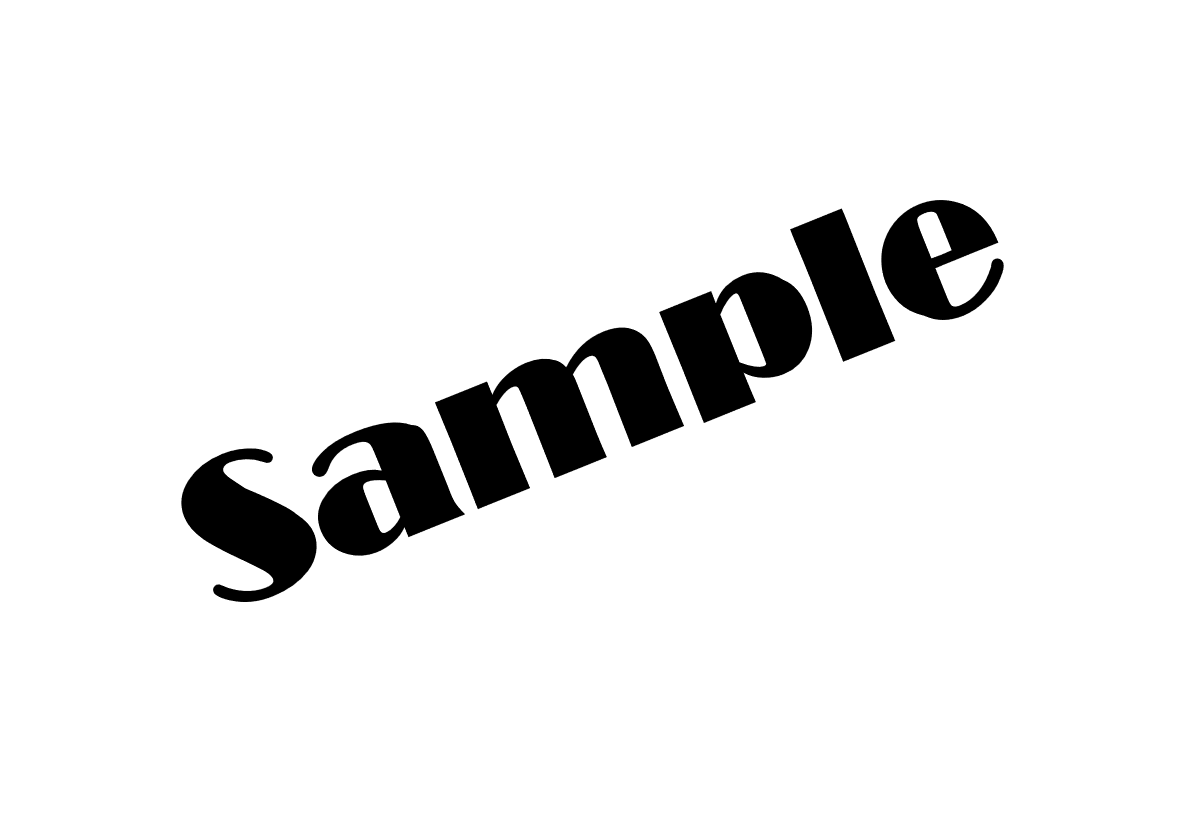
\includegraphics[scale=0.5]{image/sample.png}
    \caption{\tool の画面}
    \label{image/sample.png}
\end{figure}

\section{\tool の評価}


\section{まとめ}

\footnotesize
%%
%参考文献

\begin{thebibliography}{0}
  \bibitem{example}Example Org: "Example Title". \url{http://example.com}. アクセス日: 2021/01/31.
\end{thebibliography}

\end{document}
